\section{Project 5 - Image Restoration}
\subsection{Project Proposal}
Suppose a blurring degradation as \begin{equation} H(u,v)=\frac{T}{\pi(ua+vb)}\sin[\pi(ua+vb)]e^{-j\pi(ua+vb)} \end{equation} (a)We need to implement this blurring filter. (b)Use the filter to blur the image \emph{book\_cover.jpg} using parameters $a=b=0.1$ and $T=1$. (c)Add Gaussian noise of $N(0, 650)$ to the blurred image. (d)Restore the blurred image and the blurred noisy image using the inverse filter, Wiener filter, respectively. (e)Add Gaussian noise of 0 and different variances to the blurred image and repeat step (d), investigate the performance of the Wiener filter.

\subsection{Preliminaries}
\subsubsection{A model of the image degradation/restoration process}
\begin{equation} g(x,y)=h(x,y)\circ f(x,y)+\eta(x,y) \label{eq:degmodel_sp}\end{equation}This model shows the degradation model in spatial domain where $h(x,y)$ is the spatial representation of the degradation function and $\eta$ is a additive noise. The equivalent frequency domain representation is in \begin{equation} \label{eq:degmodel_fr} G(u,v)=H(u,v)F(u,v)+N(u,v) \end{equation} where the capital letters are the Fourier transforms of the corresponding term in Eq.\ref{eq:degmodel_sp}. The degradation is usually unknown and we have to use estimation methods. 
\subsubsection{Inverse Filtering}
In project 4, we only studied the restoration of images degraded by addictive noise. Here we talk about restoration of images degraded by degradation function $H$. A simple method is to compute estimate $\hat{F}(u,v)$ with inverse filtering by \begin{equation} \hat{F}(u,v)=\frac{G(u,v)}{H(u,v)} \end{equation} However, when we apply Eq.\ref{eq:degmodel_fr} here, we have \begin{equation} \hat{F}(u,v)=F(u,v)+\frac{H(u,v)}{H(u,v)} \end{equation} This expression tells us that even we know the exact degradation function $H$, we can not restore the original image. The smaller the value of $H$ is, the more ratio the term $N(u,v)/H(u,v)$ dominate $\hat{F}(u,v)$. One approach to settle the problem is to limit the filter frequencies to values near the origin because the values around the origin are always the highest. 
\subsubsection{Wiener filtering}
Wiener filter, also known as \emph{minimum mean square error filter} is an approach that incorporates both the degradation function and statistical characteristics of noise into the restoration process. In this approach, we consider images and noise as random variables and the objective is to find $\hat{f}$ that minimize the error $e^2=E{(f-\hat{f})^2}$. Based on some assumption, the minimum of the error function is given in the frequency domain by the expression \begin{equation}\begin{aligned} \hat{F}&=\left[ \frac{H^*(u,v)S_f(u,v)}{S_f(u,v)|H(u,v)|^2+S_{\eta}(u,v)} \right]G(u,v) \\ &=\left[\frac{H^*(u,v)}{|H(u,v)|^2+S_{\eta}(u,v)/S_f(u,v)}\right]G(u,v) \\ &=\left[ \frac{1}{H(u,v)}\frac{|H(u,v)^2|}{|H(u,v)|^2+S_{\eta}(u,v)/S_f(u,v)} \right]G(u,v) \end{aligned}\end{equation} in which $H(u,v)$ is the degradation function, $H^*(u,v)$ is the complex conjugate of $H(u,v)$, $|H(u,v)|^2$ is the squared modulus, $S_{\eta}(u,v)=|N(u,v)|^2$ and $S_f{u,v}=|F(u,v)|^2$. As we usually don't know the noise during restoration, we use a constant $K$ to substitute the term $S_n/S_f$. The value of $K$ is chosen interactively to get the best result in practice. When we set $K=0$, Wiener filtering reduces to inverse filtering.

\subsection{Experiment}
First, we use the degradation function $H$ to blur the original image Figure.\ref{fig:5_blur} and get Figure.\ref{fig:5_blur}. The result of blurring is like a motion blur. This is a characteristic of the degradation function $H$ we used here. Then we add Gaussian noise with different variance to the blurred image to verify the inverse filtering and Wiener filtering. The result is showed in Figure.\ref{fig:5_results}. In each row, we apply the same order operation: add Gaussian noise to Figure.\ref{fig:5_blur}, inverse filtering, Wiener filtering. The variance of Gaussian of each row is (650, 65, 0.06, 0) respectively. The constant parameter $K$ for Wiener filtering is set to (0.01, 0.008, 0.002, 0) for the four rows respectively.

\begin{figure}[h]
	\centering
	\begin{subfigure}[b]{0.45\linewidth}
		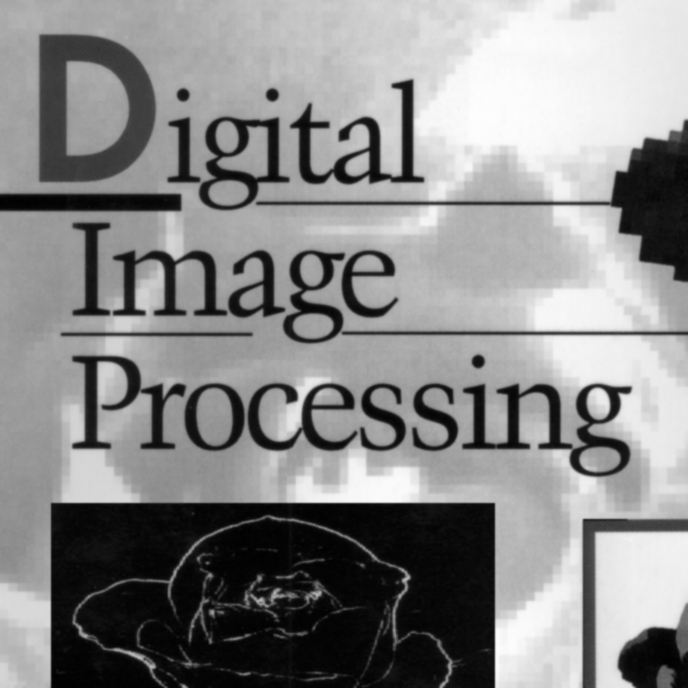
\includegraphics[width=\linewidth]{myfigure/p5/book_cover.png}
		\caption{}
		\label{fig:5_orig}
	\end{subfigure}
  	\begin{subfigure}[b]{0.45\linewidth}
		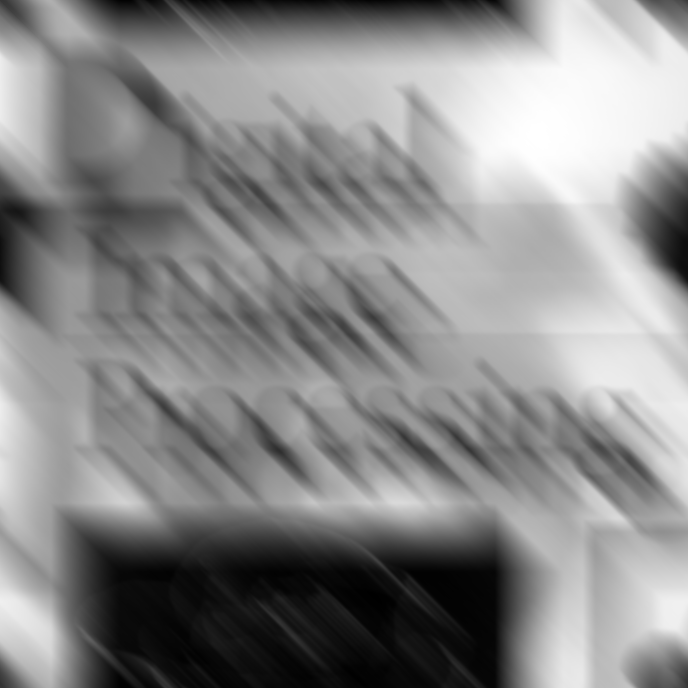
\includegraphics[width=\linewidth]{myfigure/p5/5_blur.png}
		\caption{}
		\label{fig:5_blur}
	\end{subfigure}
  	\caption{(\ref{fig:5_orig})Original test image of size $688\times 688$ pixels. (\ref{fig:5_blur})Use degradation function $H$ to blur the image.}
  	\label{fig:orig_blur}
\end{figure}

\begin{figure}[h]
	\centering
	\begin{subfigure}[b]{0.3\linewidth}
		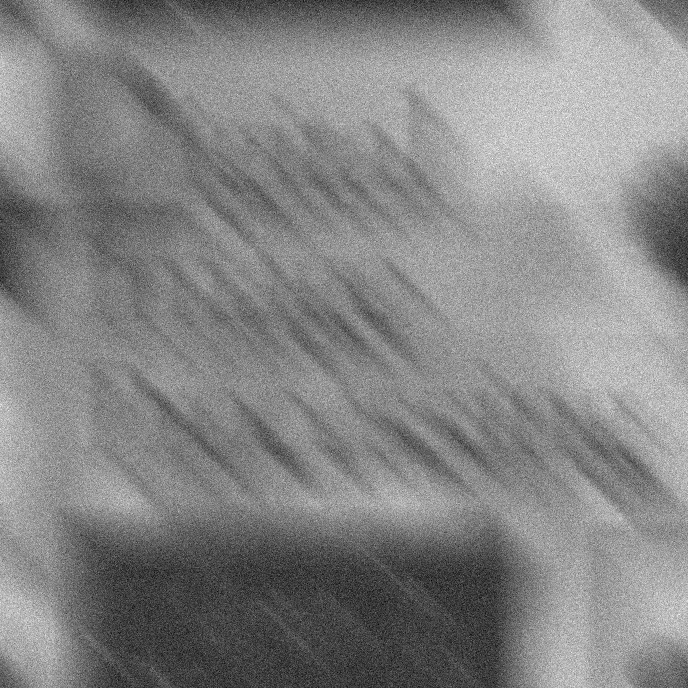
\includegraphics[width=\linewidth]{myfigure/p5/5_blur_gaussian_650.png}
		\caption{}
		\label{fig:5_gaussian_650}
	\end{subfigure}
  	\begin{subfigure}[b]{0.3\linewidth}
		
\includegraphics[width=\linewidth]{myfigure/p5/5_inverse_650.png}
		\caption{}
		\label{fig:5_inverse_650}
	\end{subfigure}
  	\begin{subfigure}[b]{0.3\linewidth}
		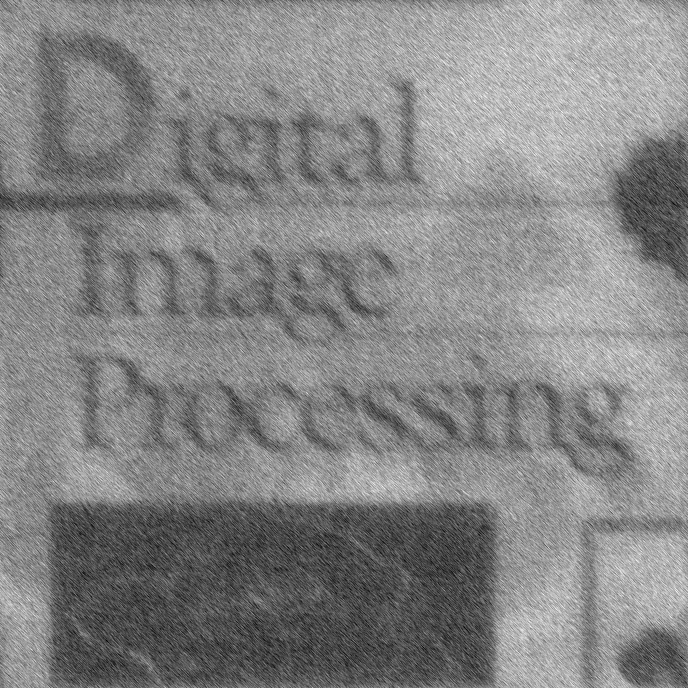
\includegraphics[width=\linewidth]{myfigure/p5/5_wiener_650.png}
		\caption{}
		\label{fig:5_wiener_650}
	\end{subfigure}
	\begin{subfigure}[b]{0.3\linewidth}
		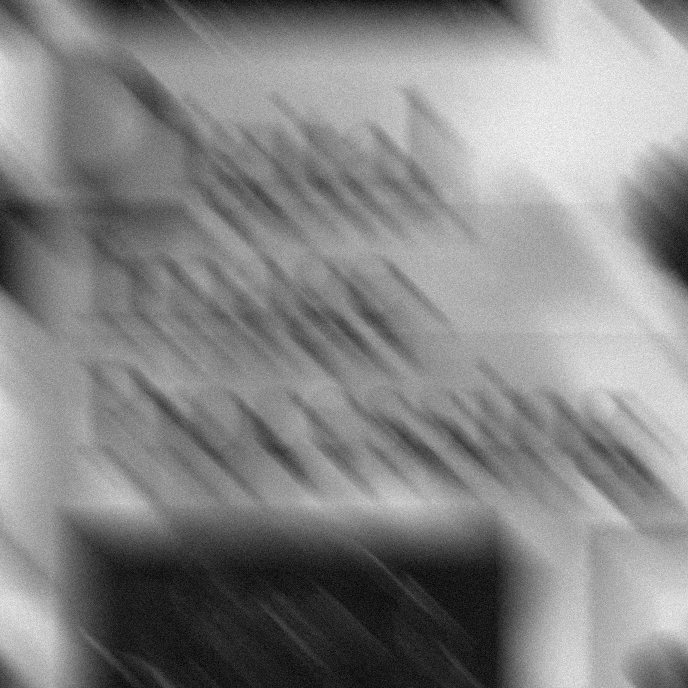
\includegraphics[width=\linewidth]{myfigure/p5/5_blur_gaussian_65.png}
		\caption{}
		\label{fig:5_gaussian_65}
	\end{subfigure}
  	\begin{subfigure}[b]{0.3\linewidth}
		
\includegraphics[width=\linewidth]{myfigure/p5/5_inverse_65.png}
		\caption{}
		\label{fig:5_inverse_65}
	\end{subfigure}
  	\begin{subfigure}[b]{0.3\linewidth}
		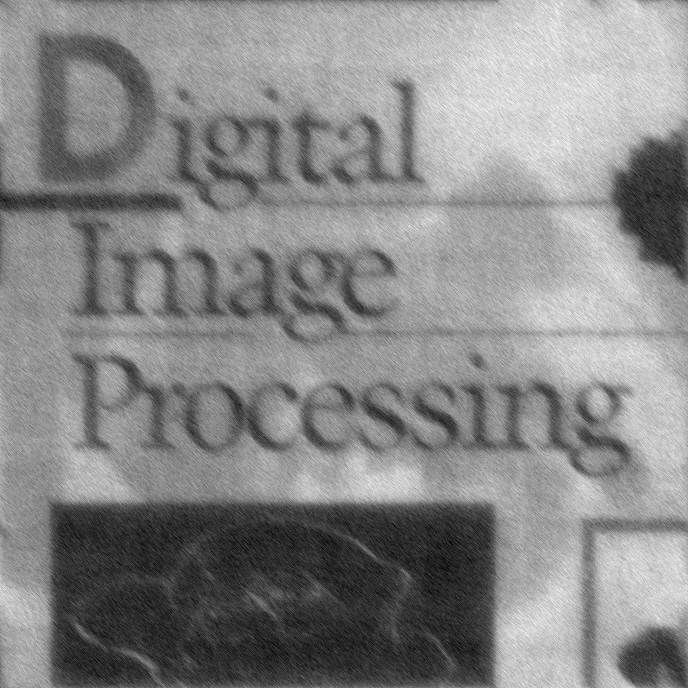
\includegraphics[width=\linewidth]{myfigure/p5/5_wiener_65.png}
		\caption{}
		\label{fig:5_wiener_65}
	\end{subfigure}
	\begin{subfigure}[b]{0.3\linewidth}
		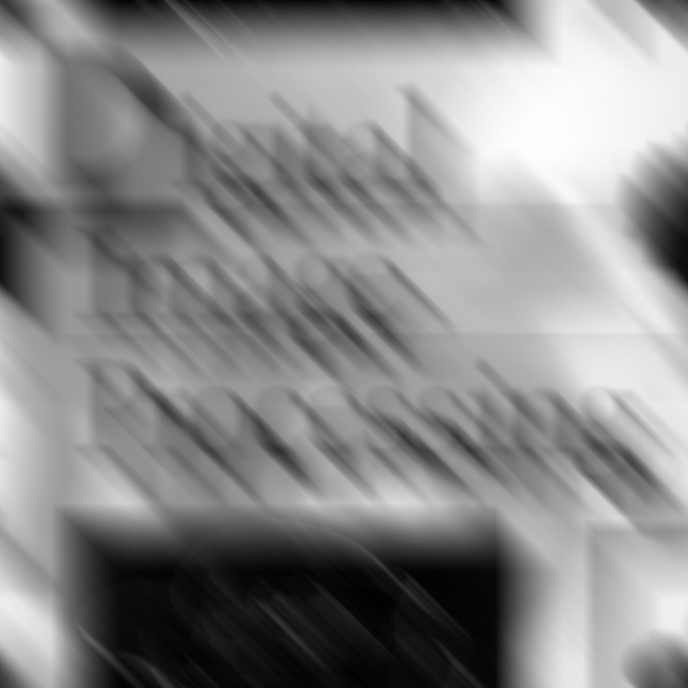
\includegraphics[width=\linewidth]{myfigure/p5/5_blur_gaussian_006.png}
		\caption{}
		\label{fig:5_gaussian_006}
	\end{subfigure}
  	\begin{subfigure}[b]{0.3\linewidth}
		
\includegraphics[width=\linewidth]{myfigure/p5/5_inverse_006.png}
		\caption{}
		\label{fig:5_inverse_006}
	\end{subfigure}
  	\begin{subfigure}[b]{0.3\linewidth}
		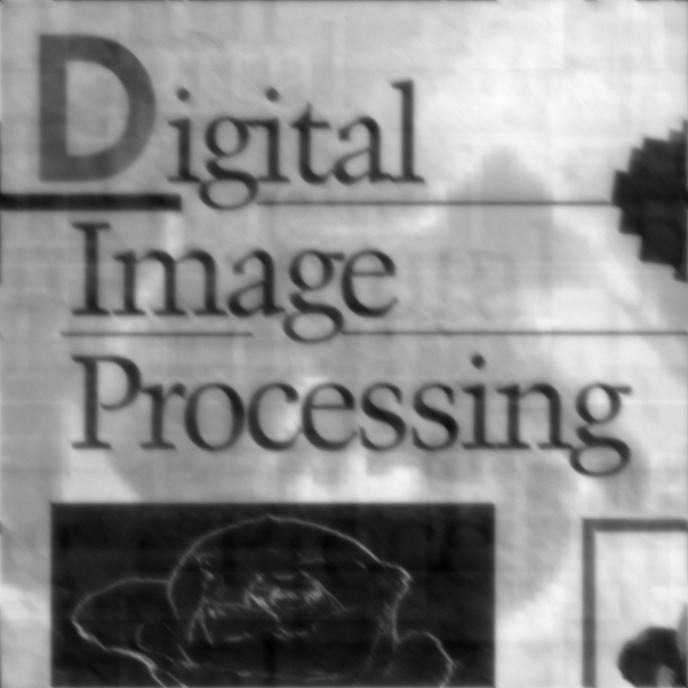
\includegraphics[width=\linewidth]{myfigure/p5/5_wiener_006.png}
		\caption{}
		\label{fig:5_wiener_006}
	\end{subfigure}
	\begin{subfigure}[b]{0.3\linewidth}
		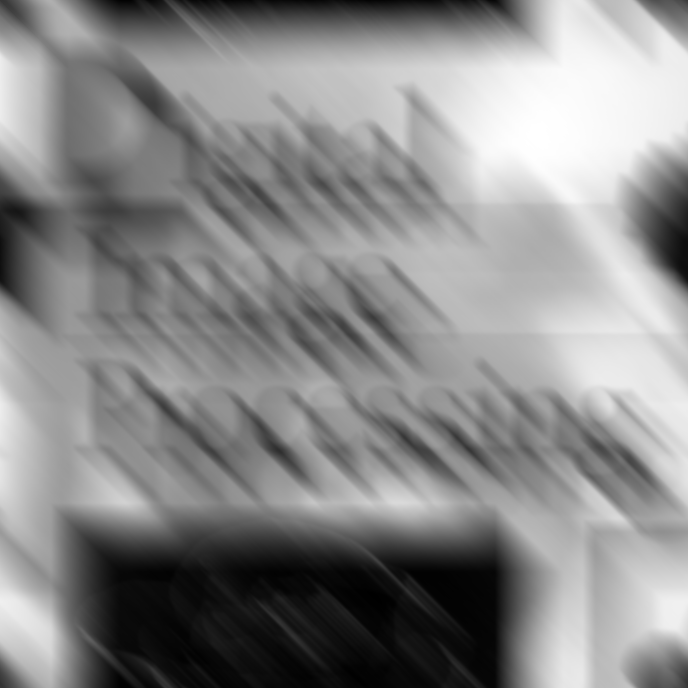
\includegraphics[width=\linewidth]{myfigure/p5/5_blur.png}
		\caption{}
		\label{fig:5_gaussian_blur}
	\end{subfigure}
  	\begin{subfigure}[b]{0.3\linewidth}
		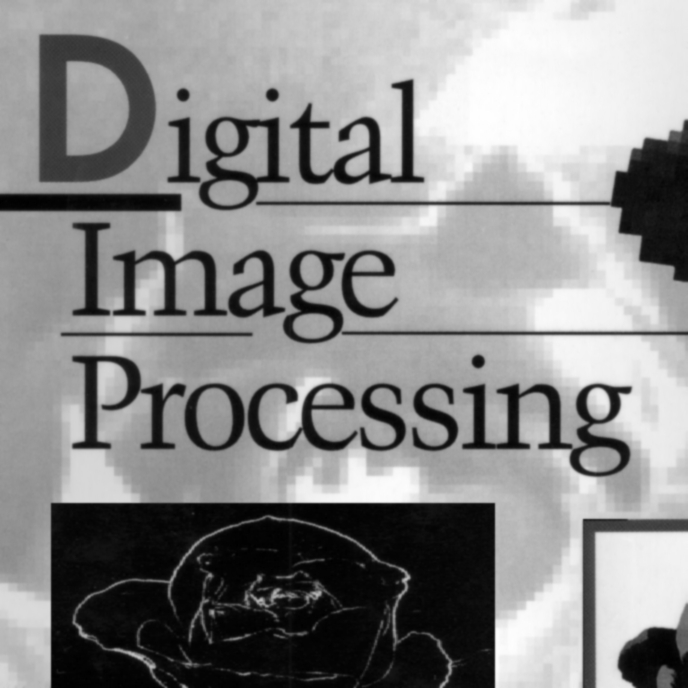
\includegraphics[width=\linewidth]{myfigure/p5/5_inverse_blur.png}
		\caption{}
		\label{fig:5_inverse_blur}
	\end{subfigure}
  	\begin{subfigure}[b]{0.3\linewidth}
		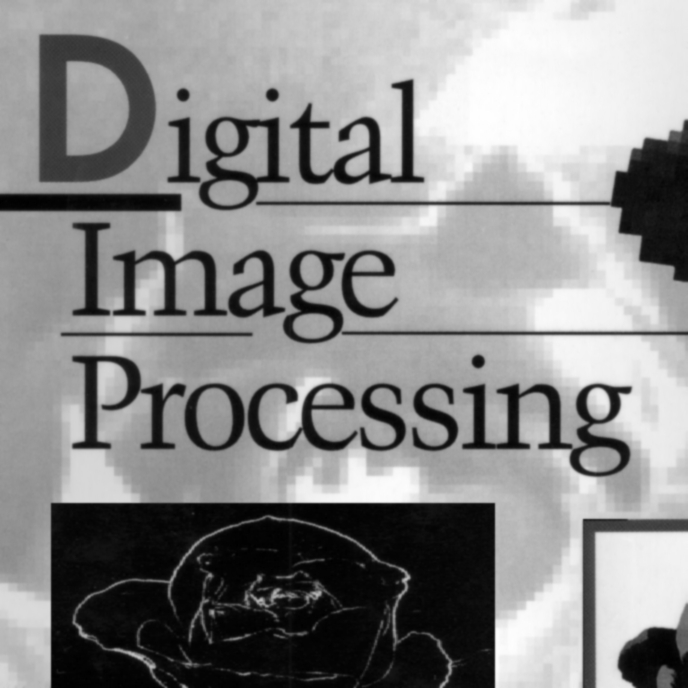
\includegraphics[width=\linewidth]{myfigure/p5/5_wiener_blur.png}
		\caption{}
		\label{fig:5_wiener_blur}
	\end{subfigure}
  	\caption{Gaussian variance of each line:(650, 65, 0.06, 0). 1st column: Blurred image with Gaussian noise. 2nd column: inverse filtering. 3rd column: Wiener filtering. Parameter $K$ for Wiener of each row: (0.01, 0.008, 0.002, 0)}
  	\label{fig:5_results}
\end{figure}

\subsection{Discussion}
In the Figure.\ref{fig:5_results}, the results of inverse filtering is as expected to be bad because of the strong inference of noise. We can see the structure is in the direction of the deblurring filter. The results of Wiener filtering is not perfect but much better than inverse filtering. The less the Gaussian variance is, the easier to get a satisfy result during manually parameter choosing. Note that the parameters used here may not be the optimal parameters because of limited search and subjective evaluation. 

\subsection{Implementation}
It seems that the implementation of this project should be easier than the prior projects. However, the fact is that without some nontrivial trick we can not get the correct process. First, do not use the intermediate result matrix for imshow() because the image may be of nonsense. Second, when do division, add a $eps$ to the denominator to avoid meaningless result. \\
The key part of implementation is listed here. Note that, I did not implement an inverse filter separately but use Wiener filter with $K=0$ as inverse filter. The common dft process function \emph{dft\_filter\_func.m} is the same as the one in project 3. The Gaussian noise generator \emph{gen\_gaussian.m} is the same as the one in project 4.

\lstset{language=Matlab} 
\begin{lstlisting}
function [ imgf ] = wiener_filter( H, K, noise, imgo )
%WIENER_FILTER wiener filter used for blurred image with noise
%   original image - imgo, degradation function H, 
%   constant of signal-to-noise ratio - K, additive noise - noise

%Sn = abs(fft2(noise)).^2;
%Sf = abs(fft2(imgo)).^2;
G = fft2(imgo).*H + fft2(noise);
H2 = abs(H) .^ 2;
%F = (H2 ./ (H .* (H2 + Sn./Sf))) .* G;
F = (H2 ./ (H .* (H2 + K))) .* G;
imgf = real(ifft2(F));
imgf = uint8(scale255(imgf));
\end{lstlisting}
\lstset{language=Matlab} 
\begin{lstlisting}
% (a) implement degradation function H
% generate basic filter
f_orig = double(f_orig);
[M, N] = size(f_orig);
% generate meshgrid
[V, U] = meshgrid(1:N, 1:M);
U = U - M/2;
V = V - N/2;
% define degradation function H
T = 1; a = 0.1; b = 0.1;
uavb = pi*( U*a + V*b + eps);
H = T./uavb .* sin( uavb ) .* exp( -1j*uavb );
H = ifftshift(H);
\end{lstlisting}

